\section{Results}

The toy model seems to indicate that the samples tend to be widely spread along directions where variance is large.
Does this make sense in terms of the gradients?
Consider a 1D normal distribution with quite small variance for the sample $x| \theta$.
If we sample $x$ far from the current mean estimate $\theta$, then due the small variance would result in large gradients, causing the result seen in fig \ref{fig:1d_low_var}. There should however be a mitigating effect due to the fact that we are unlikely to sample these far-away $x$'s and so giving smaller gradients. Experimentally this mitigation seems non-existent or inefficient, or it is something wrong with my implementation.  

\begin{figure}
\centering
  % This file was created by matplotlib2tikz v0.7.3.
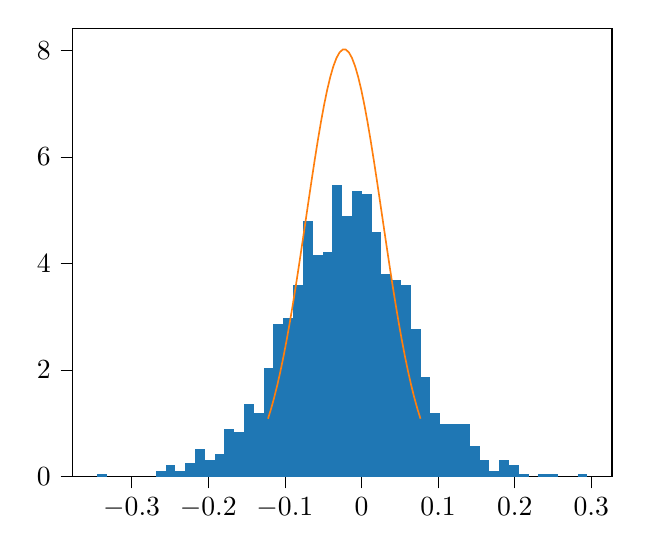
\begin{tikzpicture}

\definecolor{color0}{rgb}{0.12156862745098,0.466666666666667,0.705882352941177}
\definecolor{color1}{rgb}{1,0.498039215686275,0.0549019607843137}

\begin{axis}[
tick align=outside,
tick pos=left,
x grid style={white!69.01960784313725!black},
xmin=-0.377419363469542, xmax=0.326897716288823,
xtick style={color=black},
y grid style={white!69.01960784313725!black},
ymin=0, ymax=8.41256215782621,
ytick style={color=black}
]
\draw[fill=color0,draw opacity=0] (axis cs:-0.345404950753253,0) rectangle (axis cs:-0.332599185666737,0.052059885697002);
\draw[fill=color0,draw opacity=0] (axis cs:-0.332599185666737,0) rectangle (axis cs:-0.319793420580221,0);
\draw[fill=color0,draw opacity=0] (axis cs:-0.319793420580221,0) rectangle (axis cs:-0.306987655493705,0);
\draw[fill=color0,draw opacity=0] (axis cs:-0.306987655493705,0) rectangle (axis cs:-0.29418189040719,0);
\draw[fill=color0,draw opacity=0] (axis cs:-0.29418189040719,0) rectangle (axis cs:-0.281376125320674,0);
\draw[fill=color0,draw opacity=0] (axis cs:-0.281376125320674,0) rectangle (axis cs:-0.268570360234158,0);
\draw[fill=color0,draw opacity=0] (axis cs:-0.268570360234158,0) rectangle (axis cs:-0.255764595147642,0.104119771394004);
\draw[fill=color0,draw opacity=0] (axis cs:-0.255764595147642,0) rectangle (axis cs:-0.242958830061127,0.208239542788008);
\draw[fill=color0,draw opacity=0] (axis cs:-0.242958830061127,0) rectangle (axis cs:-0.230153064974611,0.104119771394004);
\draw[fill=color0,draw opacity=0] (axis cs:-0.230153064974611,0) rectangle (axis cs:-0.217347299888095,0.260299428485009);
\draw[fill=color0,draw opacity=0] (axis cs:-0.217347299888095,0) rectangle (axis cs:-0.204541534801579,0.520598856970019);
\draw[fill=color0,draw opacity=0] (axis cs:-0.204541534801579,0) rectangle (axis cs:-0.191735769715064,0.312359314182012);
\draw[fill=color0,draw opacity=0] (axis cs:-0.191735769715064,0) rectangle (axis cs:-0.178930004628548,0.416479085576015);
\draw[fill=color0,draw opacity=0] (axis cs:-0.178930004628548,0) rectangle (axis cs:-0.166124239542032,0.885018056849032);
\draw[fill=color0,draw opacity=0] (axis cs:-0.166124239542032,0) rectangle (axis cs:-0.153318474455517,0.83295817115203);
\draw[fill=color0,draw opacity=0] (axis cs:-0.153318474455517,0) rectangle (axis cs:-0.140512709369001,1.35355702812205);
\draw[fill=color0,draw opacity=0] (axis cs:-0.140512709369001,0) rectangle (axis cs:-0.127706944282485,1.19737737103104);
\draw[fill=color0,draw opacity=0] (axis cs:-0.127706944282485,0) rectangle (axis cs:-0.114901179195969,2.03033554218307);
\draw[fill=color0,draw opacity=0] (axis cs:-0.114901179195969,0) rectangle (axis cs:-0.102095414109454,2.8632937133351);
\draw[fill=color0,draw opacity=0] (axis cs:-0.102095414109454,0) rectangle (axis cs:-0.0892896490229378,2.96741348472911);
\draw[fill=color0,draw opacity=0] (axis cs:-0.0892896490229378,0) rectangle (axis cs:-0.0764838839364221,3.59213211309314);
\draw[fill=color0,draw opacity=0] (axis cs:-0.0764838839364221,0) rectangle (axis cs:-0.0636781188499064,4.78950948412416);
\draw[fill=color0,draw opacity=0] (axis cs:-0.0636781188499064,0) rectangle (axis cs:-0.0508723537633907,4.16479085576016);
\draw[fill=color0,draw opacity=0] (axis cs:-0.0508723537633907,0) rectangle (axis cs:-0.038066588676875,4.21685074145716);
\draw[fill=color0,draw opacity=0] (axis cs:-0.038066588676875,0) rectangle (axis cs:-0.0252608235903592,5.46628799818519);
\draw[fill=color0,draw opacity=0] (axis cs:-0.0252608235903592,0) rectangle (axis cs:-0.0124550585038435,4.89362925551819);
\draw[fill=color0,draw opacity=0] (axis cs:-0.0124550585038435,0) rectangle (axis cs:0.000350706582672278,5.36216822679118);
\draw[fill=color0,draw opacity=0] (axis cs:0.000350706582672278,0) rectangle (axis cs:0.013156471669188,5.3101083410942);
\draw[fill=color0,draw opacity=0] (axis cs:0.013156471669188,0) rectangle (axis cs:0.0259622367557037,4.58126994133616);
\draw[fill=color0,draw opacity=0] (axis cs:0.0259622367557037,0) rectangle (axis cs:0.0387680018422195,3.80037165588115);
\draw[fill=color0,draw opacity=0] (axis cs:0.0387680018422195,0) rectangle (axis cs:0.0515737669287352,3.69625188448713);
\draw[fill=color0,draw opacity=0] (axis cs:0.0515737669287352,0) rectangle (axis cs:0.0643795320152509,3.59213211309314);
\draw[fill=color0,draw opacity=0] (axis cs:0.0643795320152509,0) rectangle (axis cs:0.0771852971017666,2.75917394194111);
\draw[fill=color0,draw opacity=0] (axis cs:0.0771852971017666,0) rectangle (axis cs:0.0899910621882824,1.87415588509206);
\draw[fill=color0,draw opacity=0] (axis cs:0.0899910621882824,0) rectangle (axis cs:0.102796827274798,1.19737737103105);
\draw[fill=color0,draw opacity=0] (axis cs:0.102796827274798,0) rectangle (axis cs:0.115602592361314,0.989137828243034);
\draw[fill=color0,draw opacity=0] (axis cs:0.115602592361314,0) rectangle (axis cs:0.12840835744783,0.989137828243038);
\draw[fill=color0,draw opacity=0] (axis cs:0.12840835744783,0) rectangle (axis cs:0.141214122534345,0.989137828243034);
\draw[fill=color0,draw opacity=0] (axis cs:0.141214122534345,0) rectangle (axis cs:0.154019887620861,0.572658742667022);
\draw[fill=color0,draw opacity=0] (axis cs:0.154019887620861,0) rectangle (axis cs:0.166825652707377,0.312359314182011);
\draw[fill=color0,draw opacity=0] (axis cs:0.166825652707377,0) rectangle (axis cs:0.179631417793892,0.104119771394004);
\draw[fill=color0,draw opacity=0] (axis cs:0.179631417793892,0) rectangle (axis cs:0.192437182880408,0.312359314182011);
\draw[fill=color0,draw opacity=0] (axis cs:0.192437182880408,0) rectangle (axis cs:0.205242947966924,0.208239542788007);
\draw[fill=color0,draw opacity=0] (axis cs:0.205242947966924,0) rectangle (axis cs:0.21804871305344,0.0520598856970018);
\draw[fill=color0,draw opacity=0] (axis cs:0.21804871305344,0) rectangle (axis cs:0.230854478139955,0);
\draw[fill=color0,draw opacity=0] (axis cs:0.230854478139955,0) rectangle (axis cs:0.243660243226471,0.0520598856970018);
\draw[fill=color0,draw opacity=0] (axis cs:0.243660243226471,0) rectangle (axis cs:0.256466008312987,0.0520598856970018);
\draw[fill=color0,draw opacity=0] (axis cs:0.256466008312987,0) rectangle (axis cs:0.269271773399503,0);
\draw[fill=color0,draw opacity=0] (axis cs:0.269271773399503,0) rectangle (axis cs:0.282077538486018,0);
\draw[fill=color0,draw opacity=0] (axis cs:0.282077538486018,0) rectangle (axis cs:0.294883303572534,0.052059885697002);
\addplot [semithick, color1]
table {%
-0.12202716854655 1.08520499624329
-0.117965792259979 1.27341499854328
-0.113904415973407 1.48434223974259
-0.109843039686836 1.71871568808433
-0.105781663400265 1.97687835045291
-0.101720287113693 2.25871667891995
-0.0976589108271218 2.56359538818518
-0.0935975345405504 2.89030127041828
-0.089536158253979 3.23699967094385
-0.0854747819674077 3.60120716916907
-0.0814134056808363 3.97978367462426
-0.0773520293942649 4.36894659096945
-0.0732906531076935 4.76430892899306
-0.0692292768211221 5.16094228656203
-0.0651679005345507 5.5534644986725
-0.0611065242479794 5.93615054832781
-0.057045147961408 6.30306408506911
-0.0529837716748366 6.64820569685094
-0.0489223953882652 6.96567300005029
-0.0448610191016938 7.24982672682687
-0.0407996428151224 7.49545636576185
-0.0367382665285511 7.69793860395083
-0.0326768902419797 7.85338186133036
-0.0286155139554083 7.95875061382071
-0.0245541376688369 8.01196395983449
-0.0204927613822655 8.01196395983449
-0.0164313850956941 7.95875061382071
-0.0123700088091227 7.85338186133036
-0.00830863252255136 7.69793860395083
-0.00424725623597998 7.49545636576185
-0.000185879949408593 7.24982672682687
0.00387549633716279 6.96567300005029
0.00793687262373417 6.64820569685094
0.0119982489103056 6.30306408506911
0.0160596251968769 5.93615054832782
0.0201210014834483 5.55346449867251
0.0241823777700197 5.16094228656203
0.0282437540565911 4.76430892899306
0.0323051303431625 4.36894659096945
0.0363665066297339 3.97978367462426
0.0404278829163052 3.60120716916908
0.0444892592028766 3.23699967094385
0.048550635489448 2.89030127041828
0.0526120117760194 2.56359538818518
0.0566733880625908 2.25871667891996
0.0607347643491622 1.97687835045291
0.0647961406357335 1.71871568808433
0.0688575169223049 1.48434223974259
0.0729188932088763 1.27341499854328
0.0769802694954477 1.08520499624329
};
\end{axis}

\end{tikzpicture}
  \caption{1D, $\sigma^2 = 1/4$}\label{fig:1d_low_var}
\end{figure}

\begin{figure}
\centering
  % This file was created by matplotlib2tikz v0.7.3.
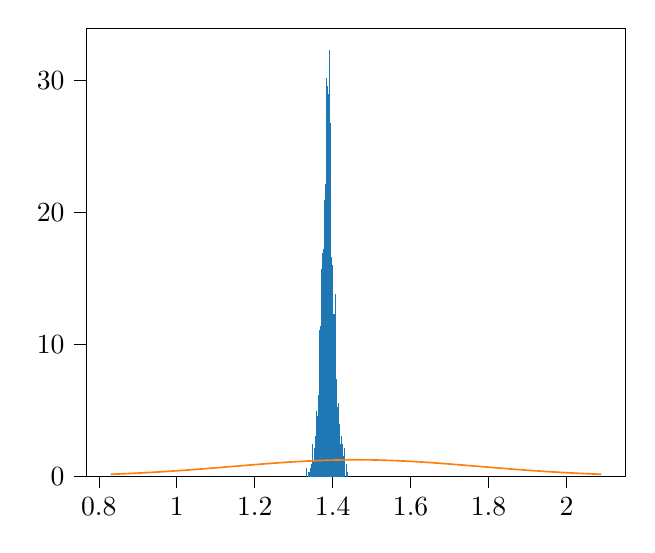
\begin{tikzpicture}

\definecolor{color0}{rgb}{0.12156862745098,0.466666666666667,0.705882352941177}
\definecolor{color1}{rgb}{1,0.498039215686275,0.0549019607843137}

\begin{axis}[
tick align=outside,
tick pos=left,
x grid style={white!69.01960784313725!black},
xmin=0.767568748149515, xmax=2.15206565431013,
xtick style={color=black},
y grid style={white!69.01960784313725!black},
ymin=0, ymax=33.9289042621717,
ytick style={color=black}
]
\draw[fill=color0,draw opacity=0] (axis cs:1.33136491688426,0) rectangle (axis cs:1.33353121142274,0.615490326751415);
\draw[fill=color0,draw opacity=0] (axis cs:1.33353121142274,0) rectangle (axis cs:1.33569750596123,0);
\draw[fill=color0,draw opacity=0] (axis cs:1.33569750596123,0) rectangle (axis cs:1.33786380049972,0.307745163375707);
\draw[fill=color0,draw opacity=0] (axis cs:1.33786380049972,0) rectangle (axis cs:1.34003009503821,0.307745163375707);
\draw[fill=color0,draw opacity=0] (axis cs:1.34003009503821,0) rectangle (axis cs:1.34219638957669,0.307745163375707);
\draw[fill=color0,draw opacity=0] (axis cs:1.34219638957669,0) rectangle (axis cs:1.34436268411518,0.615490326751352);
\draw[fill=color0,draw opacity=0] (axis cs:1.34436268411518,0) rectangle (axis cs:1.34652897865367,0.923235490127122);
\draw[fill=color0,draw opacity=0] (axis cs:1.34652897865367,0) rectangle (axis cs:1.34869527319216,2.46196130700566);
\draw[fill=color0,draw opacity=0] (axis cs:1.34869527319216,0) rectangle (axis cs:1.35086156773064,1.2309806535027);
\draw[fill=color0,draw opacity=0] (axis cs:1.35086156773064,0) rectangle (axis cs:1.35302786226913,2.15421614362995);
\draw[fill=color0,draw opacity=0] (axis cs:1.35302786226913,0) rectangle (axis cs:1.35519415680762,1.84647098025424);
\draw[fill=color0,draw opacity=0] (axis cs:1.35519415680762,0) rectangle (axis cs:1.35736045134611,3.07745163375707);
\draw[fill=color0,draw opacity=0] (axis cs:1.35736045134611,0) rectangle (axis cs:1.35952674588459,4.92392261401081);
\draw[fill=color0,draw opacity=0] (axis cs:1.35952674588459,0) rectangle (axis cs:1.36169304042308,4.61617745063561);
\draw[fill=color0,draw opacity=0] (axis cs:1.36169304042308,0) rectangle (axis cs:1.36385933496157,6.15490326751415);
\draw[fill=color0,draw opacity=0] (axis cs:1.36385933496157,0) rectangle (axis cs:1.36602562950005,7.69362908439268);
\draw[fill=color0,draw opacity=0] (axis cs:1.36602562950005,0) rectangle (axis cs:1.36819192403854,11.0788258815243);
\draw[fill=color0,draw opacity=0] (axis cs:1.36819192403854,0) rectangle (axis cs:1.37035821857703,11.3865710449012);
\draw[fill=color0,draw opacity=0] (axis cs:1.37035821857703,0) rectangle (axis cs:1.37252451311552,15.6950033321611);
\draw[fill=color0,draw opacity=0] (axis cs:1.37252451311552,0) rectangle (axis cs:1.374690807654,16.9259839856622);
\draw[fill=color0,draw opacity=0] (axis cs:1.374690807654,0) rectangle (axis cs:1.37685710219249,17.2337291490396);
\draw[fill=color0,draw opacity=0] (axis cs:1.37685710219249,0) rectangle (axis cs:1.37902339673098,20.9266711095481);
\draw[fill=color0,draw opacity=0] (axis cs:1.37902339673098,0) rectangle (axis cs:1.38118969126947,20.9266711095481);
\draw[fill=color0,draw opacity=0] (axis cs:1.38118969126947,0) rectangle (axis cs:1.38335598580795,22.1576517630487);
\draw[fill=color0,draw opacity=0] (axis cs:1.38335598580795,0) rectangle (axis cs:1.38552228034644,30.1590260108193);
\draw[fill=color0,draw opacity=0] (axis cs:1.38552228034644,0) rectangle (axis cs:1.38768857488493,29.5435356840679);
\draw[fill=color0,draw opacity=0] (axis cs:1.38768857488493,0) rectangle (axis cs:1.38985486942342,28.9280453573135);
\draw[fill=color0,draw opacity=0] (axis cs:1.38985486942342,0) rectangle (axis cs:1.3920211639619,32.3132421544493);
\draw[fill=color0,draw opacity=0] (axis cs:1.3920211639619,0) rectangle (axis cs:1.39418745850039,26.7738292136865);
\draw[fill=color0,draw opacity=0] (axis cs:1.39418745850039,0) rectangle (axis cs:1.39635375303888,22.7731420898023);
\draw[fill=color0,draw opacity=0] (axis cs:1.39635375303888,0) rectangle (axis cs:1.39852004757736,16.6182388222865);
\draw[fill=color0,draw opacity=0] (axis cs:1.39852004757736,0) rectangle (axis cs:1.40068634211585,16.0027484955368);
\draw[fill=color0,draw opacity=0] (axis cs:1.40068634211585,0) rectangle (axis cs:1.40285263665434,12.3098065350283);
\draw[fill=color0,draw opacity=0] (axis cs:1.40285263665434,0) rectangle (axis cs:1.40501893119283,12.3098065350283);
\draw[fill=color0,draw opacity=0] (axis cs:1.40501893119283,0) rectangle (axis cs:1.40718522573131,13.8485323519054);
\draw[fill=color0,draw opacity=0] (axis cs:1.40718522573131,0) rectangle (axis cs:1.4093515202698,9.54010006464692);
\draw[fill=color0,draw opacity=0] (axis cs:1.4093515202698,0) rectangle (axis cs:1.41151781480829,7.38588392101698);
\draw[fill=color0,draw opacity=0] (axis cs:1.41151781480829,0) rectangle (axis cs:1.41368410934678,5.23166777738649);
\draw[fill=color0,draw opacity=0] (axis cs:1.41368410934678,0) rectangle (axis cs:1.41585040388526,5.53941294076273);
\draw[fill=color0,draw opacity=0] (axis cs:1.41585040388526,0) rectangle (axis cs:1.41801669842375,4.00068712388419);
\draw[fill=color0,draw opacity=0] (axis cs:1.41801669842375,0) rectangle (axis cs:1.42018299296224,2.46196130700566);
\draw[fill=color0,draw opacity=0] (axis cs:1.42018299296224,0) rectangle (axis cs:1.42234928750073,3.07745163375676);
\draw[fill=color0,draw opacity=0] (axis cs:1.42234928750073,0) rectangle (axis cs:1.42451558203921,1.84647098025424);
\draw[fill=color0,draw opacity=0] (axis cs:1.42451558203921,0) rectangle (axis cs:1.4266818765777,2.46196130700566);
\draw[fill=color0,draw opacity=0] (axis cs:1.4266818765777,0) rectangle (axis cs:1.42884817111619,1.53872581687838);
\draw[fill=color0,draw opacity=0] (axis cs:1.42884817111619,0) rectangle (axis cs:1.43101446565467,2.15421614362995);
\draw[fill=color0,draw opacity=0] (axis cs:1.43101446565467,0) rectangle (axis cs:1.43318076019316,0);
\draw[fill=color0,draw opacity=0] (axis cs:1.43318076019316,0) rectangle (axis cs:1.43534705473165,0.923235490127122);
\draw[fill=color0,draw opacity=0] (axis cs:1.43534705473165,0) rectangle (axis cs:1.43751334927014,0);
\draw[fill=color0,draw opacity=0] (axis cs:1.43751334927014,0) rectangle (axis cs:1.43967964380862,0.307745163375707);
\addplot [semithick, color1]
table {%
0.83050042570227 0.171585975816163
0.856186824703395 0.201344590100837
0.881873223704519 0.234695115239114
0.907559622705644 0.2717528112305
0.933246021706769 0.312571912225388
0.958932420707893 0.357134464719914
0.984618819709018 0.405340021288434
1.01030521871014 0.45699675693
1.03599161771127 0.511814587269907
1.06167801671239 0.569400849035079
1.08736441571352 0.629259050328356
1.11305081471464 0.690791110154575
1.13873721371577 0.753303384614774
1.16442361271689 0.816016624910671
1.19011001171801 0.878079836034513
1.21579641071914 0.938587813318666
1.24148280972026 0.996601937341185
1.26716920872139 1.05117361776779
1.29285560772251 1.10136960580485
1.31854200672364 1.14629825491681
1.34422840572476 1.18513571091078
1.36991480472589 1.21715096383107
1.39560120372701 1.24172870084283
1.42128760272814 1.25838896344683
1.44697400172926 1.26680273221294
1.47266040073039 1.26680273221294
1.49834679973151 1.25838896344683
1.52403319873263 1.24172870084283
1.54971959773376 1.21715096383107
1.57540599673488 1.18513571091078
1.60109239573601 1.14629825491681
1.62677879473713 1.10136960580485
1.65246519373826 1.05117361776779
1.67815159273938 0.996601937341185
1.70383799174051 0.938587813318666
1.72952439074163 0.878079836034512
1.75521078974276 0.81601662491067
1.78089718874388 0.753303384614774
1.80658358774501 0.690791110154575
1.83226998674613 0.629259050328356
1.85795638574725 0.569400849035078
1.88364278474838 0.511814587269907
1.9093291837495 0.45699675693
1.93501558275063 0.405340021288433
1.96070198175175 0.357134464719914
1.98638838075288 0.312571912225388
2.012074779754 0.2717528112305
2.03776117875513 0.234695115239114
2.06344757775625 0.201344590100838
2.08913397675738 0.171585975816162
};
\end{axis}

\end{tikzpicture}

  \caption{1D, $\sigma^2 = 10$}\label{fig:1d_high_var}
\end{figure}

% \begin{figure}
%   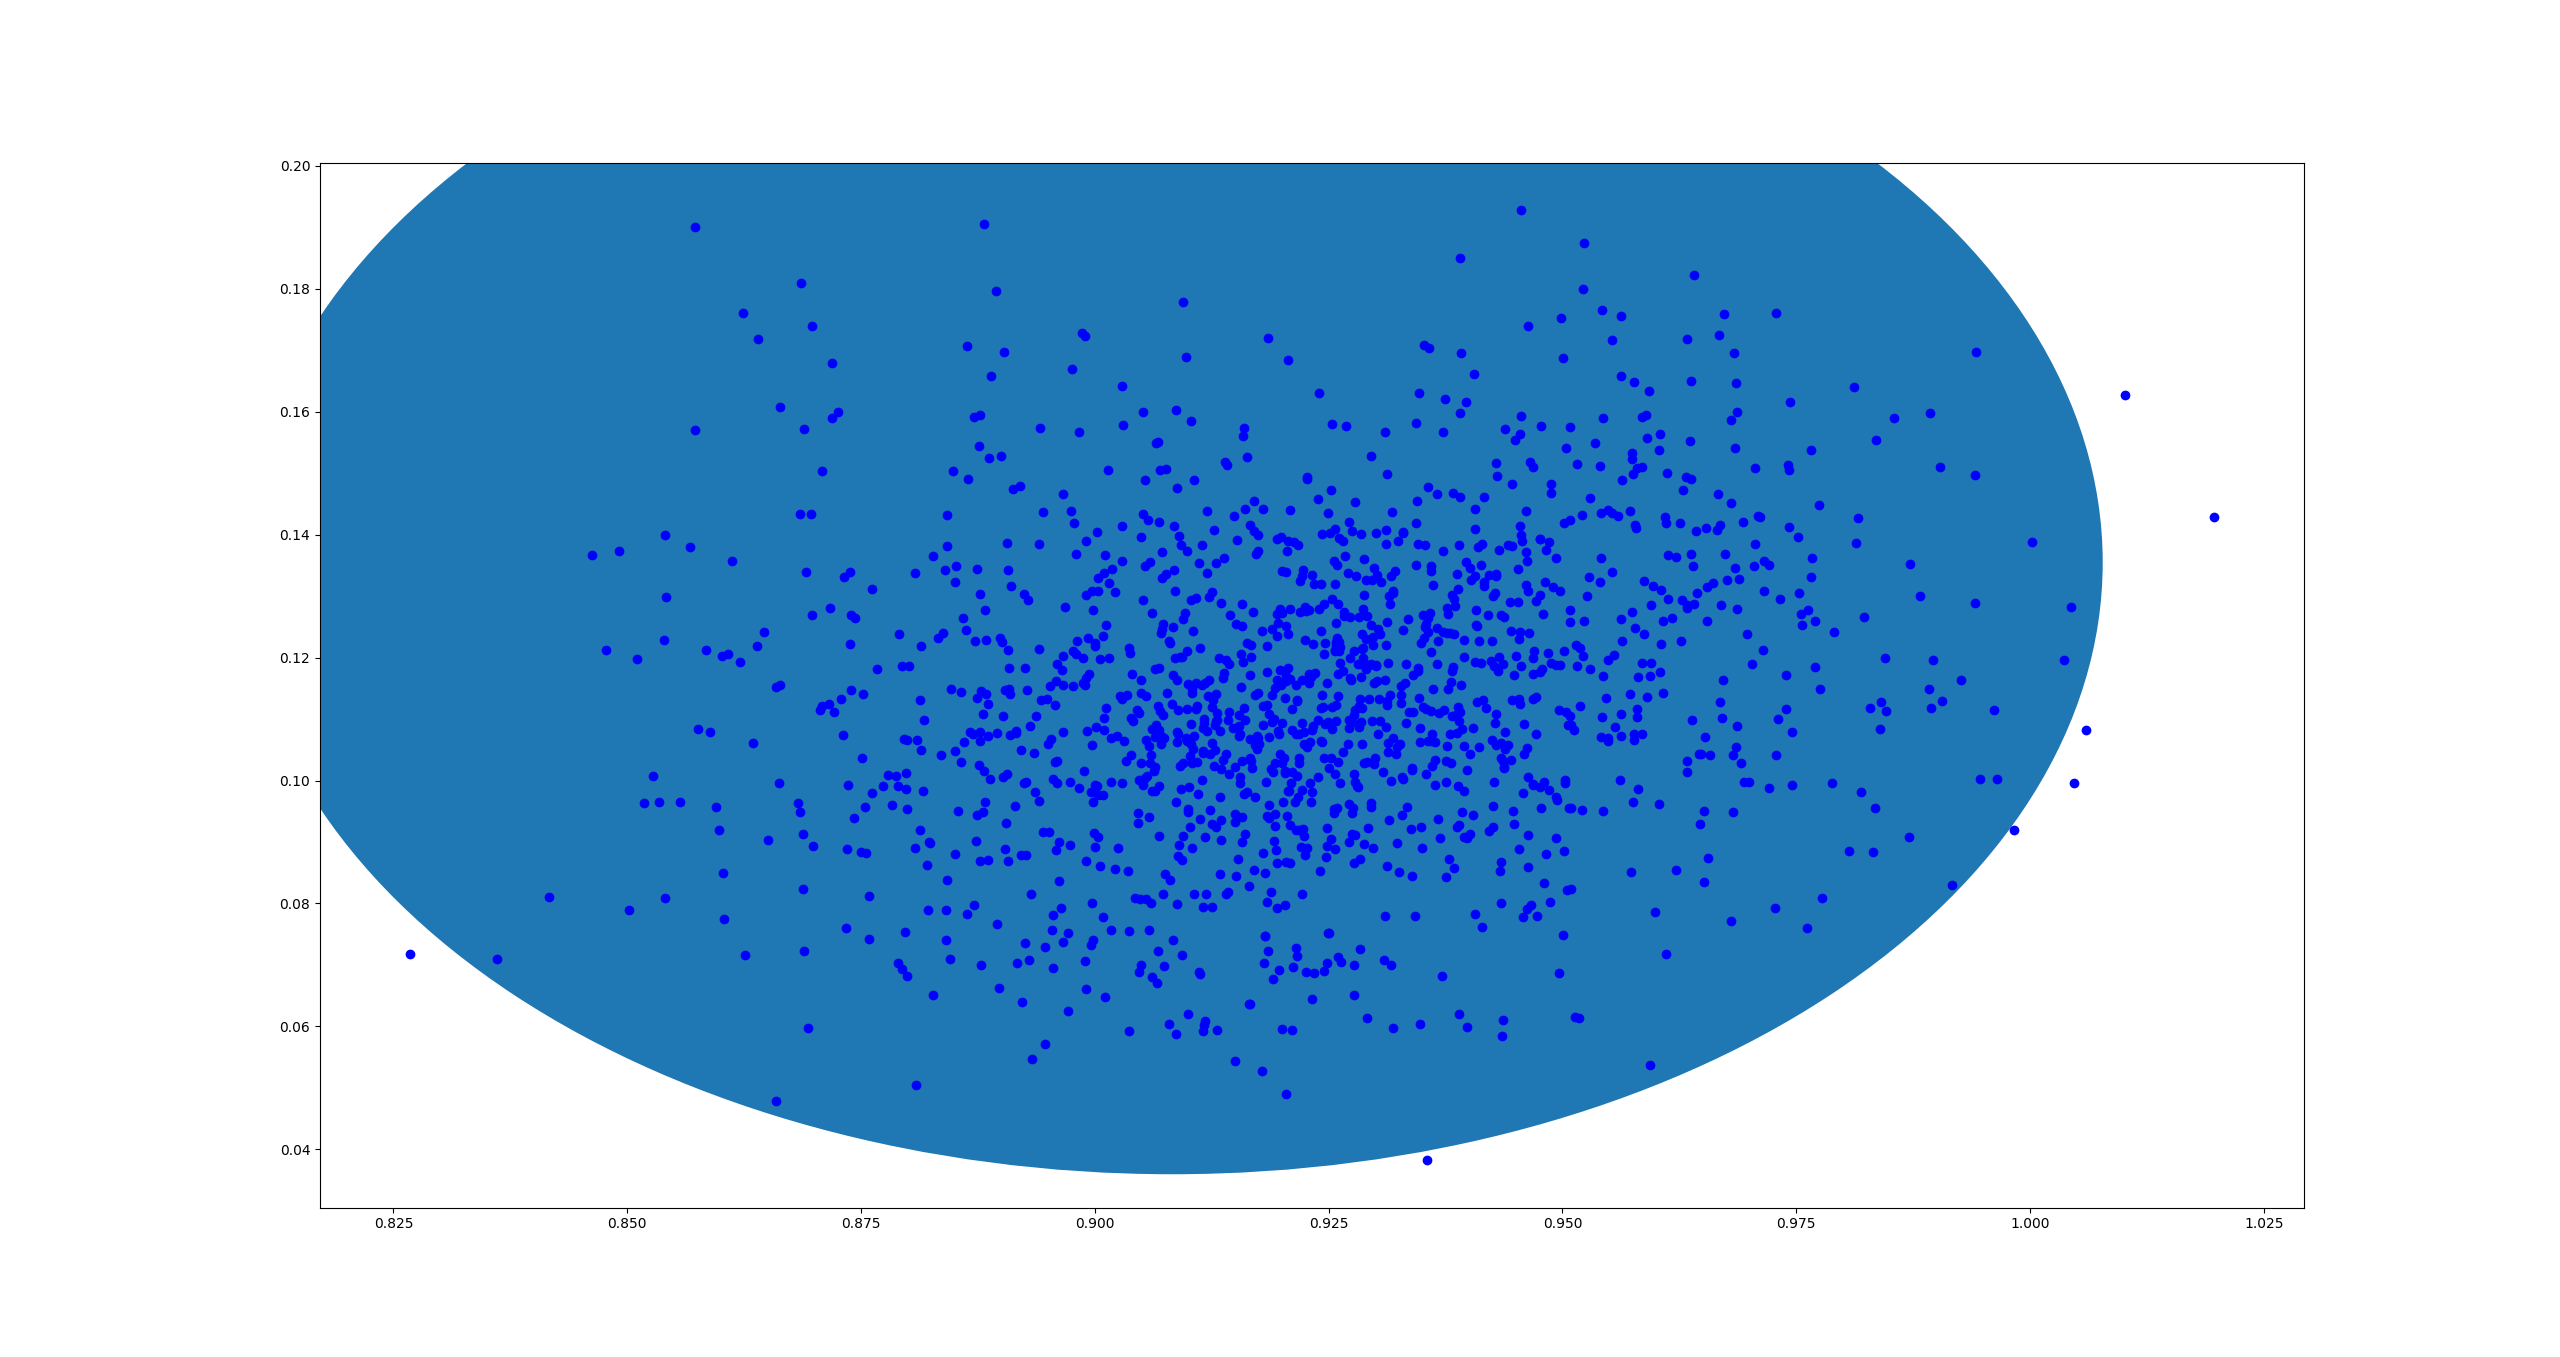
\includegraphics[width=\linewidth]{fig/spherical_cov.png}
%   \caption{Bivariate, spherical cov}\label{fig:spherical_cov}
% \end{figure}


\begin{figure}
\centering
  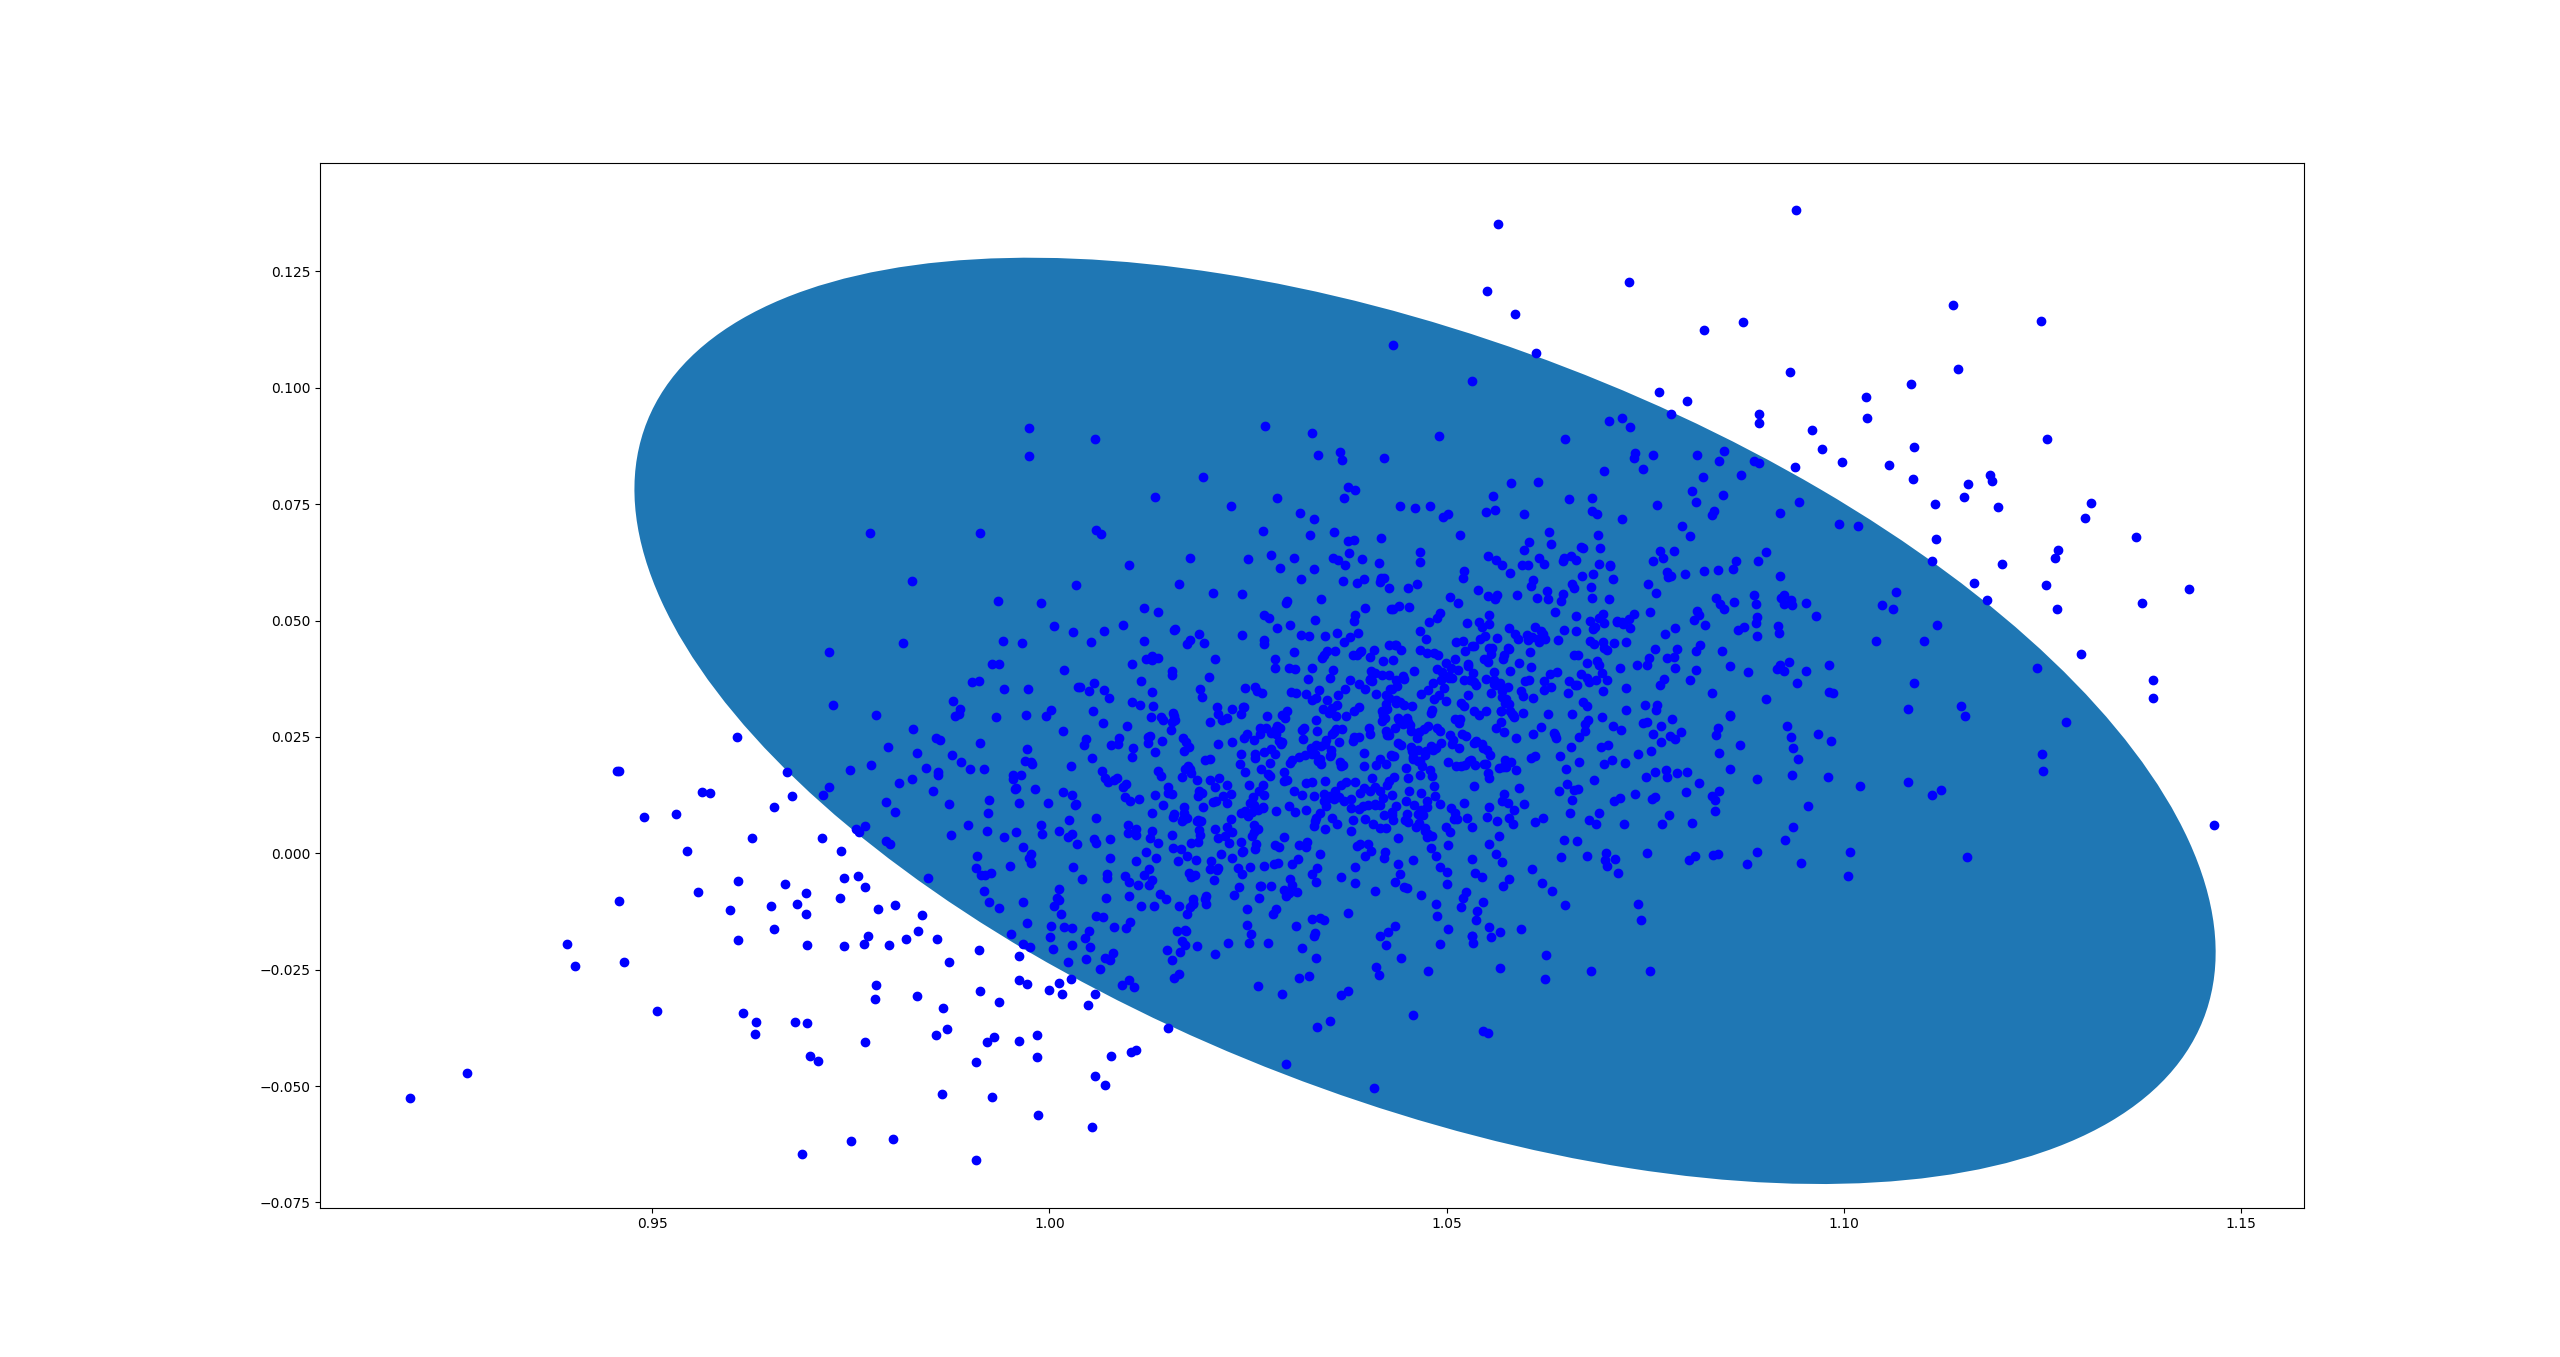
\includegraphics[width=\linewidth]{fig/mirrored_cov_1.png}
  \caption{Bivariate, correlated}\label{fig:mirrored_cov_1}
\end{figure}
